% Generado por floyd.c
\documentclass[a4paper,11pt]{article}
\usepackage[utf8]{inputenc}
\usepackage{tikz}
\usepackage{array}
\usepackage[table]{xcolor}
\usepackage{longtable}
\usepackage{geometry}
\geometry{margin=1.5cm}
\begin{document}
\begin{center}
{\LARGE \textbf{Proyecto 1: Rutas Óptimas (Algoritmo de Floyd)}}\\[2cm]
{\large Investigación de Operaciones\\[2cm]
{\large Integrantes: }\\[1cm]
{\large Jose Pablo Fernandez Jimenez - 2023117752}\\[1cm]
{\large Diego Durán Rodríguez - 2022437509}\\[2cm]
{\large Segundo semestre 2025\\[1cm]
\end{center}
\newpage
\section*{Algoritmo de Floyd}


     Robert W. Floyd nació el 8 de junio de 1936 en New York, Estados Unidos y falleció el 25 de septiembre de 2001. Fue un importante científico de la computación y recibió un Turing Award en 1978 por sus contribuciones a la teoría de lenguajes de programación, algoritmos y estructuras de datos. Estudió Artes Liberales y Física en la Universidad de Chicago y realizó publicaciones muy influyentes en el campo de la informática. Uno de sus trabajos más importantes fue el desarrollo del algoritmo de Floyd-Warshall en 1962~\cite{hosch2024}.

El algoritmo de Floyd es un algoritmo de grafos con el cual se puede encontrar la ruta más corta entre todos los pares de nodos en un grafo ponderado. Este algoritmo tiene complejidad temporal $O(n^3)$ y espacial $O(n^2)$, donde $n$ es el número de nodos en el grafo. Para llevar a cabo el cálculo de la ruta más corta, el algoritmo utiliza dos matrices: una matriz de distancias (D) y una matriz de predecesores (P), que muestra el camino más corto~\cite{mukhopadhyay2023}.

\bigskip
\section*{Problema}
\begin{center}
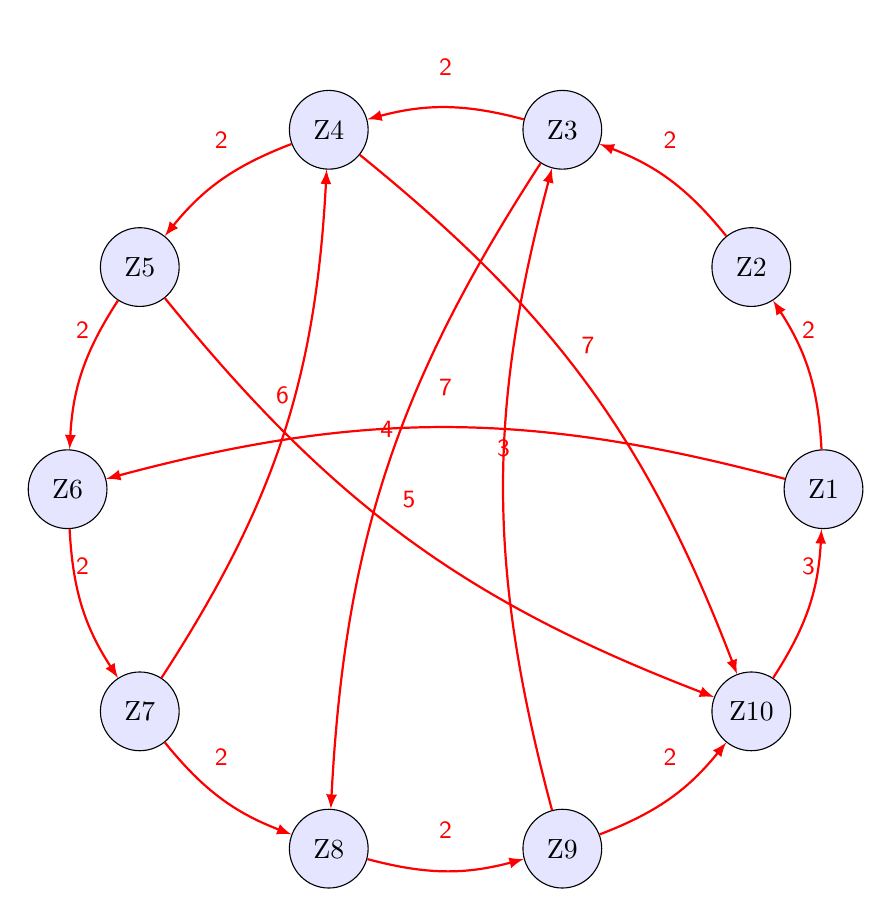
\begin{tikzpicture}[scale=1.2,
  every node/.style={circle, draw, fill=blue!10, minimum size=10mm},
  every edge/.style={draw, thick}]
\node (N0) at (4.000, 0.000) {Z1};
\node (N1) at (3.236, 2.351) {Z2};
\node (N2) at (1.236, 3.804) {Z3};
\node (N3) at (-1.236, 3.804) {Z4};
\node (N4) at (-3.236, 2.351) {Z5};
\node (N5) at (-4.000, 0.000) {Z6};
\node (N6) at (-3.236, -2.351) {Z7};
\node (N7) at (-1.236, -3.804) {Z8};
\node (N8) at (1.236, -3.804) {Z9};
\node (N9) at (3.236, -2.351) {Z10};
\draw[->, thick, >=latex, red] (N0) to[bend right=15] node[midway, above, draw=none, fill=none, rectangle, font=\small\sffamily] {2} (N1);
\draw[->, thick, >=latex, red] (N0) to[bend right=15] node[midway, above, draw=none, fill=none, rectangle, font=\small\sffamily] {7} (N5);
\draw[->, thick, >=latex, red] (N1) to[bend right=15] node[midway, above, draw=none, fill=none, rectangle, font=\small\sffamily] {2} (N2);
\draw[->, thick, >=latex, red] (N2) to[bend right=15] node[midway, above, draw=none, fill=none, rectangle, font=\small\sffamily] {2} (N3);
\draw[->, thick, >=latex, red] (N2) to[bend right=15] node[midway, above, draw=none, fill=none, rectangle, font=\small\sffamily] {4} (N7);
\draw[->, thick, >=latex, red] (N3) to[bend right=15] node[midway, above, draw=none, fill=none, rectangle, font=\small\sffamily] {2} (N4);
\draw[->, thick, >=latex, red] (N3) to[bend left=15] node[midway, above, draw=none, fill=none, rectangle, font=\small\sffamily] {7} (N9);
\draw[->, thick, >=latex, red] (N4) to[bend right=15] node[midway, above, draw=none, fill=none, rectangle, font=\small\sffamily] {2} (N5);
\draw[->, thick, >=latex, red] (N4) to[bend right=15] node[midway, above, draw=none, fill=none, rectangle, font=\small\sffamily] {5} (N9);
\draw[->, thick, >=latex, red] (N5) to[bend right=15] node[midway, above, draw=none, fill=none, rectangle, font=\small\sffamily] {2} (N6);
\draw[->, thick, >=latex, red] (N6) to[bend right=15] node[midway, above, draw=none, fill=none, rectangle, font=\small\sffamily] {6} (N3);
\draw[->, thick, >=latex, red] (N6) to[bend right=15] node[midway, above, draw=none, fill=none, rectangle, font=\small\sffamily] {2} (N7);
\draw[->, thick, >=latex, red] (N7) to[bend right=15] node[midway, above, draw=none, fill=none, rectangle, font=\small\sffamily] {2} (N8);
\draw[->, thick, >=latex, red] (N8) to[bend left=15] node[midway, above, draw=none, fill=none, rectangle, font=\small\sffamily] {3} (N2);
\draw[->, thick, >=latex, red] (N8) to[bend right=15] node[midway, above, draw=none, fill=none, rectangle, font=\small\sffamily] {2} (N9);
\draw[->, thick, >=latex, red] (N9) to[bend right=15] node[midway, above, draw=none, fill=none, rectangle, font=\small\sffamily] {3} (N0);
\end{tikzpicture}
\end{center}
\newpage
\section*{Tablas iniciales}
\subsection*{D(0)}
\begin{center}
\begin{tabular}{c|cccccccccc}
 & Z1 & Z2 & Z3 & Z4 & Z5 & Z6 & Z7 & Z8 & Z9 & Z10 \\ \hline
Z1 & 0 & 2 & $\infty$ & $\infty$ & $\infty$ & 7 & $\infty$ & $\infty$ & $\infty$ & $\infty$ \\
Z2 & $\infty$ & 0 & 2 & $\infty$ & $\infty$ & $\infty$ & $\infty$ & $\infty$ & $\infty$ & $\infty$ \\
Z3 & $\infty$ & $\infty$ & 0 & 2 & $\infty$ & $\infty$ & $\infty$ & 4 & $\infty$ & $\infty$ \\
Z4 & $\infty$ & $\infty$ & $\infty$ & 0 & 2 & $\infty$ & $\infty$ & $\infty$ & $\infty$ & 7 \\
Z5 & $\infty$ & $\infty$ & $\infty$ & $\infty$ & 0 & 2 & $\infty$ & $\infty$ & $\infty$ & 5 \\
Z6 & $\infty$ & $\infty$ & $\infty$ & $\infty$ & $\infty$ & 0 & 2 & $\infty$ & $\infty$ & $\infty$ \\
Z7 & $\infty$ & $\infty$ & $\infty$ & 6 & $\infty$ & $\infty$ & 0 & 2 & $\infty$ & $\infty$ \\
Z8 & $\infty$ & $\infty$ & $\infty$ & $\infty$ & $\infty$ & $\infty$ & $\infty$ & 0 & 2 & $\infty$ \\
Z9 & $\infty$ & $\infty$ & 3 & $\infty$ & $\infty$ & $\infty$ & $\infty$ & $\infty$ & 0 & 2 \\
Z10 & 3 & $\infty$ & $\infty$ & $\infty$ & $\infty$ & $\infty$ & $\infty$ & $\infty$ & $\infty$ & 0 \\
\end{tabular}
\end{center}
\subsection*{P(0)}
\begin{center}
\begin{tabular}{c|cccccccccc}
 & Z1 & Z2 & Z3 & Z4 & Z5 & Z6 & Z7 & Z8 & Z9 & Z10 \\ \hline
Z1 & 0 & 0 & 0 & 0 & 0 & 0 & 0 & 0 & 0 & 0 \\
Z2 & 0 & 0 & 0 & 0 & 0 & 0 & 0 & 0 & 0 & 0 \\
Z3 & 0 & 0 & 0 & 0 & 0 & 0 & 0 & 0 & 0 & 0 \\
Z4 & 0 & 0 & 0 & 0 & 0 & 0 & 0 & 0 & 0 & 0 \\
Z5 & 0 & 0 & 0 & 0 & 0 & 0 & 0 & 0 & 0 & 0 \\
Z6 & 0 & 0 & 0 & 0 & 0 & 0 & 0 & 0 & 0 & 0 \\
Z7 & 0 & 0 & 0 & 0 & 0 & 0 & 0 & 0 & 0 & 0 \\
Z8 & 0 & 0 & 0 & 0 & 0 & 0 & 0 & 0 & 0 & 0 \\
Z9 & 0 & 0 & 0 & 0 & 0 & 0 & 0 & 0 & 0 & 0 \\
Z10 & 0 & 0 & 0 & 0 & 0 & 0 & 0 & 0 & 0 & 0 \\
\end{tabular}
\end{center}
\newpage
\section*{Tablas intermedias}
\section*{Cálculo de D(1)}
\subsection*{D(1)}
\begin{center}
\begin{tabular}{c|cccccccccc}
 & Z1 & Z2 & Z3 & Z4 & Z5 & Z6 & Z7 & Z8 & Z9 & Z10 \\ \hline
Z1 & 0 & 2 & $\infty$ & $\infty$ & $\infty$ & 7 & $\infty$ & $\infty$ & $\infty$ & $\infty$ \\
Z2 & $\infty$ & 0 & 2 & $\infty$ & $\infty$ & $\infty$ & $\infty$ & $\infty$ & $\infty$ & $\infty$ \\
Z3 & $\infty$ & $\infty$ & 0 & 2 & $\infty$ & $\infty$ & $\infty$ & 4 & $\infty$ & $\infty$ \\
Z4 & $\infty$ & $\infty$ & $\infty$ & 0 & 2 & $\infty$ & $\infty$ & $\infty$ & $\infty$ & 7 \\
Z5 & $\infty$ & $\infty$ & $\infty$ & $\infty$ & 0 & 2 & $\infty$ & $\infty$ & $\infty$ & 5 \\
Z6 & $\infty$ & $\infty$ & $\infty$ & $\infty$ & $\infty$ & 0 & 2 & $\infty$ & $\infty$ & $\infty$ \\
Z7 & $\infty$ & $\infty$ & $\infty$ & 6 & $\infty$ & $\infty$ & 0 & 2 & $\infty$ & $\infty$ \\
Z8 & $\infty$ & $\infty$ & $\infty$ & $\infty$ & $\infty$ & $\infty$ & $\infty$ & 0 & 2 & $\infty$ \\
Z9 & $\infty$ & $\infty$ & 3 & $\infty$ & $\infty$ & $\infty$ & $\infty$ & $\infty$ & 0 & 2 \\
Z10 & 3 & \textcolor{orange}{5} & $\infty$ & $\infty$ & $\infty$ & \textcolor{orange}{10} & $\infty$ & $\infty$ & $\infty$ & 0 \\
\end{tabular}
\end{center}
\subsection*{P(1)}
\begin{center}
\begin{tabular}{c|cccccccccc}
 & Z1 & Z2 & Z3 & Z4 & Z5 & Z6 & Z7 & Z8 & Z9 & Z10 \\ \hline
Z1 & 0 & 0 & 0 & 0 & 0 & 0 & 0 & 0 & 0 & 0 \\
Z2 & 0 & 0 & 0 & 0 & 0 & 0 & 0 & 0 & 0 & 0 \\
Z3 & 0 & 0 & 0 & 0 & 0 & 0 & 0 & 0 & 0 & 0 \\
Z4 & 0 & 0 & 0 & 0 & 0 & 0 & 0 & 0 & 0 & 0 \\
Z5 & 0 & 0 & 0 & 0 & 0 & 0 & 0 & 0 & 0 & 0 \\
Z6 & 0 & 0 & 0 & 0 & 0 & 0 & 0 & 0 & 0 & 0 \\
Z7 & 0 & 0 & 0 & 0 & 0 & 0 & 0 & 0 & 0 & 0 \\
Z8 & 0 & 0 & 0 & 0 & 0 & 0 & 0 & 0 & 0 & 0 \\
Z9 & 0 & 0 & 0 & 0 & 0 & 0 & 0 & 0 & 0 & 0 \\
Z10 & 0 & Z1 & 0 & 0 & 0 & Z1 & 0 & 0 & 0 & 0 \\
\end{tabular}
\end{center}
\newpage
\section*{Cálculo de D(2)}
\subsection*{D(2)}
\begin{center}
\begin{tabular}{c|cccccccccc}
 & Z1 & Z2 & Z3 & Z4 & Z5 & Z6 & Z7 & Z8 & Z9 & Z10 \\ \hline
Z1 & 0 & 2 & \textcolor{orange}{4} & $\infty$ & $\infty$ & 7 & $\infty$ & $\infty$ & $\infty$ & $\infty$ \\
Z2 & $\infty$ & 0 & 2 & $\infty$ & $\infty$ & $\infty$ & $\infty$ & $\infty$ & $\infty$ & $\infty$ \\
Z3 & $\infty$ & $\infty$ & 0 & 2 & $\infty$ & $\infty$ & $\infty$ & 4 & $\infty$ & $\infty$ \\
Z4 & $\infty$ & $\infty$ & $\infty$ & 0 & 2 & $\infty$ & $\infty$ & $\infty$ & $\infty$ & 7 \\
Z5 & $\infty$ & $\infty$ & $\infty$ & $\infty$ & 0 & 2 & $\infty$ & $\infty$ & $\infty$ & 5 \\
Z6 & $\infty$ & $\infty$ & $\infty$ & $\infty$ & $\infty$ & 0 & 2 & $\infty$ & $\infty$ & $\infty$ \\
Z7 & $\infty$ & $\infty$ & $\infty$ & 6 & $\infty$ & $\infty$ & 0 & 2 & $\infty$ & $\infty$ \\
Z8 & $\infty$ & $\infty$ & $\infty$ & $\infty$ & $\infty$ & $\infty$ & $\infty$ & 0 & 2 & $\infty$ \\
Z9 & $\infty$ & $\infty$ & 3 & $\infty$ & $\infty$ & $\infty$ & $\infty$ & $\infty$ & 0 & 2 \\
Z10 & 3 & 5 & \textcolor{orange}{7} & $\infty$ & $\infty$ & 10 & $\infty$ & $\infty$ & $\infty$ & 0 \\
\end{tabular}
\end{center}
\subsection*{P(2)}
\begin{center}
\begin{tabular}{c|cccccccccc}
 & Z1 & Z2 & Z3 & Z4 & Z5 & Z6 & Z7 & Z8 & Z9 & Z10 \\ \hline
Z1 & 0 & 0 & Z2 & 0 & 0 & 0 & 0 & 0 & 0 & 0 \\
Z2 & 0 & 0 & 0 & 0 & 0 & 0 & 0 & 0 & 0 & 0 \\
Z3 & 0 & 0 & 0 & 0 & 0 & 0 & 0 & 0 & 0 & 0 \\
Z4 & 0 & 0 & 0 & 0 & 0 & 0 & 0 & 0 & 0 & 0 \\
Z5 & 0 & 0 & 0 & 0 & 0 & 0 & 0 & 0 & 0 & 0 \\
Z6 & 0 & 0 & 0 & 0 & 0 & 0 & 0 & 0 & 0 & 0 \\
Z7 & 0 & 0 & 0 & 0 & 0 & 0 & 0 & 0 & 0 & 0 \\
Z8 & 0 & 0 & 0 & 0 & 0 & 0 & 0 & 0 & 0 & 0 \\
Z9 & 0 & 0 & 0 & 0 & 0 & 0 & 0 & 0 & 0 & 0 \\
Z10 & 0 & Z1 & Z2 & 0 & 0 & Z1 & 0 & 0 & 0 & 0 \\
\end{tabular}
\end{center}
\newpage
\section*{Cálculo de D(3)}
\subsection*{D(3)}
\begin{center}
\begin{tabular}{c|cccccccccc}
 & Z1 & Z2 & Z3 & Z4 & Z5 & Z6 & Z7 & Z8 & Z9 & Z10 \\ \hline
Z1 & 0 & 2 & 4 & \textcolor{orange}{6} & $\infty$ & 7 & $\infty$ & \textcolor{orange}{8} & $\infty$ & $\infty$ \\
Z2 & $\infty$ & 0 & 2 & \textcolor{orange}{4} & $\infty$ & $\infty$ & $\infty$ & \textcolor{orange}{6} & $\infty$ & $\infty$ \\
Z3 & $\infty$ & $\infty$ & 0 & 2 & $\infty$ & $\infty$ & $\infty$ & 4 & $\infty$ & $\infty$ \\
Z4 & $\infty$ & $\infty$ & $\infty$ & 0 & 2 & $\infty$ & $\infty$ & $\infty$ & $\infty$ & 7 \\
Z5 & $\infty$ & $\infty$ & $\infty$ & $\infty$ & 0 & 2 & $\infty$ & $\infty$ & $\infty$ & 5 \\
Z6 & $\infty$ & $\infty$ & $\infty$ & $\infty$ & $\infty$ & 0 & 2 & $\infty$ & $\infty$ & $\infty$ \\
Z7 & $\infty$ & $\infty$ & $\infty$ & 6 & $\infty$ & $\infty$ & 0 & 2 & $\infty$ & $\infty$ \\
Z8 & $\infty$ & $\infty$ & $\infty$ & $\infty$ & $\infty$ & $\infty$ & $\infty$ & 0 & 2 & $\infty$ \\
Z9 & $\infty$ & $\infty$ & 3 & \textcolor{orange}{5} & $\infty$ & $\infty$ & $\infty$ & \textcolor{orange}{7} & 0 & 2 \\
Z10 & 3 & 5 & 7 & \textcolor{orange}{9} & $\infty$ & 10 & $\infty$ & \textcolor{orange}{11} & $\infty$ & 0 \\
\end{tabular}
\end{center}
\subsection*{P(3)}
\begin{center}
\begin{tabular}{c|cccccccccc}
 & Z1 & Z2 & Z3 & Z4 & Z5 & Z6 & Z7 & Z8 & Z9 & Z10 \\ \hline
Z1 & 0 & 0 & Z2 & Z3 & 0 & 0 & 0 & Z3 & 0 & 0 \\
Z2 & 0 & 0 & 0 & Z3 & 0 & 0 & 0 & Z3 & 0 & 0 \\
Z3 & 0 & 0 & 0 & 0 & 0 & 0 & 0 & 0 & 0 & 0 \\
Z4 & 0 & 0 & 0 & 0 & 0 & 0 & 0 & 0 & 0 & 0 \\
Z5 & 0 & 0 & 0 & 0 & 0 & 0 & 0 & 0 & 0 & 0 \\
Z6 & 0 & 0 & 0 & 0 & 0 & 0 & 0 & 0 & 0 & 0 \\
Z7 & 0 & 0 & 0 & 0 & 0 & 0 & 0 & 0 & 0 & 0 \\
Z8 & 0 & 0 & 0 & 0 & 0 & 0 & 0 & 0 & 0 & 0 \\
Z9 & 0 & 0 & 0 & Z3 & 0 & 0 & 0 & Z3 & 0 & 0 \\
Z10 & 0 & Z1 & Z2 & Z3 & 0 & Z1 & 0 & Z3 & 0 & 0 \\
\end{tabular}
\end{center}
\newpage
\section*{Cálculo de D(4)}
\subsection*{D(4)}
\begin{center}
\begin{tabular}{c|cccccccccc}
 & Z1 & Z2 & Z3 & Z4 & Z5 & Z6 & Z7 & Z8 & Z9 & Z10 \\ \hline
Z1 & 0 & 2 & 4 & 6 & \textcolor{orange}{8} & 7 & $\infty$ & 8 & $\infty$ & \textcolor{orange}{13} \\
Z2 & $\infty$ & 0 & 2 & 4 & \textcolor{orange}{6} & $\infty$ & $\infty$ & 6 & $\infty$ & \textcolor{orange}{11} \\
Z3 & $\infty$ & $\infty$ & 0 & 2 & \textcolor{orange}{4} & $\infty$ & $\infty$ & 4 & $\infty$ & \textcolor{orange}{9} \\
Z4 & $\infty$ & $\infty$ & $\infty$ & 0 & 2 & $\infty$ & $\infty$ & $\infty$ & $\infty$ & 7 \\
Z5 & $\infty$ & $\infty$ & $\infty$ & $\infty$ & 0 & 2 & $\infty$ & $\infty$ & $\infty$ & 5 \\
Z6 & $\infty$ & $\infty$ & $\infty$ & $\infty$ & $\infty$ & 0 & 2 & $\infty$ & $\infty$ & $\infty$ \\
Z7 & $\infty$ & $\infty$ & $\infty$ & 6 & \textcolor{orange}{8} & $\infty$ & 0 & 2 & $\infty$ & \textcolor{orange}{13} \\
Z8 & $\infty$ & $\infty$ & $\infty$ & $\infty$ & $\infty$ & $\infty$ & $\infty$ & 0 & 2 & $\infty$ \\
Z9 & $\infty$ & $\infty$ & 3 & 5 & \textcolor{orange}{7} & $\infty$ & $\infty$ & 7 & 0 & 2 \\
Z10 & 3 & 5 & 7 & 9 & \textcolor{orange}{11} & 10 & $\infty$ & 11 & $\infty$ & 0 \\
\end{tabular}
\end{center}
\subsection*{P(4)}
\begin{center}
\begin{tabular}{c|cccccccccc}
 & Z1 & Z2 & Z3 & Z4 & Z5 & Z6 & Z7 & Z8 & Z9 & Z10 \\ \hline
Z1 & 0 & 0 & Z2 & Z3 & Z4 & 0 & 0 & Z3 & 0 & Z4 \\
Z2 & 0 & 0 & 0 & Z3 & Z4 & 0 & 0 & Z3 & 0 & Z4 \\
Z3 & 0 & 0 & 0 & 0 & Z4 & 0 & 0 & 0 & 0 & Z4 \\
Z4 & 0 & 0 & 0 & 0 & 0 & 0 & 0 & 0 & 0 & 0 \\
Z5 & 0 & 0 & 0 & 0 & 0 & 0 & 0 & 0 & 0 & 0 \\
Z6 & 0 & 0 & 0 & 0 & 0 & 0 & 0 & 0 & 0 & 0 \\
Z7 & 0 & 0 & 0 & 0 & Z4 & 0 & 0 & 0 & 0 & Z4 \\
Z8 & 0 & 0 & 0 & 0 & 0 & 0 & 0 & 0 & 0 & 0 \\
Z9 & 0 & 0 & 0 & Z3 & Z4 & 0 & 0 & Z3 & 0 & 0 \\
Z10 & 0 & Z1 & Z2 & Z3 & Z4 & Z1 & 0 & Z3 & 0 & 0 \\
\end{tabular}
\end{center}
\newpage
\section*{Cálculo de D(5)}
\subsection*{D(5)}
\begin{center}
\begin{tabular}{c|cccccccccc}
 & Z1 & Z2 & Z3 & Z4 & Z5 & Z6 & Z7 & Z8 & Z9 & Z10 \\ \hline
Z1 & 0 & 2 & 4 & 6 & 8 & 7 & $\infty$ & 8 & $\infty$ & 13 \\
Z2 & $\infty$ & 0 & 2 & 4 & 6 & \textcolor{orange}{8} & $\infty$ & 6 & $\infty$ & 11 \\
Z3 & $\infty$ & $\infty$ & 0 & 2 & 4 & \textcolor{orange}{6} & $\infty$ & 4 & $\infty$ & 9 \\
Z4 & $\infty$ & $\infty$ & $\infty$ & 0 & 2 & \textcolor{orange}{4} & $\infty$ & $\infty$ & $\infty$ & 7 \\
Z5 & $\infty$ & $\infty$ & $\infty$ & $\infty$ & 0 & 2 & $\infty$ & $\infty$ & $\infty$ & 5 \\
Z6 & $\infty$ & $\infty$ & $\infty$ & $\infty$ & $\infty$ & 0 & 2 & $\infty$ & $\infty$ & $\infty$ \\
Z7 & $\infty$ & $\infty$ & $\infty$ & 6 & 8 & \textcolor{orange}{10} & 0 & 2 & $\infty$ & 13 \\
Z8 & $\infty$ & $\infty$ & $\infty$ & $\infty$ & $\infty$ & $\infty$ & $\infty$ & 0 & 2 & $\infty$ \\
Z9 & $\infty$ & $\infty$ & 3 & 5 & 7 & \textcolor{orange}{9} & $\infty$ & 7 & 0 & 2 \\
Z10 & 3 & 5 & 7 & 9 & 11 & 10 & $\infty$ & 11 & $\infty$ & 0 \\
\end{tabular}
\end{center}
\subsection*{P(5)}
\begin{center}
\begin{tabular}{c|cccccccccc}
 & Z1 & Z2 & Z3 & Z4 & Z5 & Z6 & Z7 & Z8 & Z9 & Z10 \\ \hline
Z1 & 0 & 0 & Z2 & Z3 & Z4 & 0 & 0 & Z3 & 0 & Z4 \\
Z2 & 0 & 0 & 0 & Z3 & Z4 & Z5 & 0 & Z3 & 0 & Z4 \\
Z3 & 0 & 0 & 0 & 0 & Z4 & Z5 & 0 & 0 & 0 & Z4 \\
Z4 & 0 & 0 & 0 & 0 & 0 & Z5 & 0 & 0 & 0 & 0 \\
Z5 & 0 & 0 & 0 & 0 & 0 & 0 & 0 & 0 & 0 & 0 \\
Z6 & 0 & 0 & 0 & 0 & 0 & 0 & 0 & 0 & 0 & 0 \\
Z7 & 0 & 0 & 0 & 0 & Z4 & Z5 & 0 & 0 & 0 & Z4 \\
Z8 & 0 & 0 & 0 & 0 & 0 & 0 & 0 & 0 & 0 & 0 \\
Z9 & 0 & 0 & 0 & Z3 & Z4 & Z5 & 0 & Z3 & 0 & 0 \\
Z10 & 0 & Z1 & Z2 & Z3 & Z4 & Z1 & 0 & Z3 & 0 & 0 \\
\end{tabular}
\end{center}
\newpage
\section*{Cálculo de D(6)}
\subsection*{D(6)}
\begin{center}
\begin{tabular}{c|cccccccccc}
 & Z1 & Z2 & Z3 & Z4 & Z5 & Z6 & Z7 & Z8 & Z9 & Z10 \\ \hline
Z1 & 0 & 2 & 4 & 6 & 8 & 7 & \textcolor{orange}{9} & 8 & $\infty$ & 13 \\
Z2 & $\infty$ & 0 & 2 & 4 & 6 & 8 & \textcolor{orange}{10} & 6 & $\infty$ & 11 \\
Z3 & $\infty$ & $\infty$ & 0 & 2 & 4 & 6 & \textcolor{orange}{8} & 4 & $\infty$ & 9 \\
Z4 & $\infty$ & $\infty$ & $\infty$ & 0 & 2 & 4 & \textcolor{orange}{6} & $\infty$ & $\infty$ & 7 \\
Z5 & $\infty$ & $\infty$ & $\infty$ & $\infty$ & 0 & 2 & \textcolor{orange}{4} & $\infty$ & $\infty$ & 5 \\
Z6 & $\infty$ & $\infty$ & $\infty$ & $\infty$ & $\infty$ & 0 & 2 & $\infty$ & $\infty$ & $\infty$ \\
Z7 & $\infty$ & $\infty$ & $\infty$ & 6 & 8 & 10 & 0 & 2 & $\infty$ & 13 \\
Z8 & $\infty$ & $\infty$ & $\infty$ & $\infty$ & $\infty$ & $\infty$ & $\infty$ & 0 & 2 & $\infty$ \\
Z9 & $\infty$ & $\infty$ & 3 & 5 & 7 & 9 & \textcolor{orange}{11} & 7 & 0 & 2 \\
Z10 & 3 & 5 & 7 & 9 & 11 & 10 & \textcolor{orange}{12} & 11 & $\infty$ & 0 \\
\end{tabular}
\end{center}
\subsection*{P(6)}
\begin{center}
\begin{tabular}{c|cccccccccc}
 & Z1 & Z2 & Z3 & Z4 & Z5 & Z6 & Z7 & Z8 & Z9 & Z10 \\ \hline
Z1 & 0 & 0 & Z2 & Z3 & Z4 & 0 & Z6 & Z3 & 0 & Z4 \\
Z2 & 0 & 0 & 0 & Z3 & Z4 & Z5 & Z6 & Z3 & 0 & Z4 \\
Z3 & 0 & 0 & 0 & 0 & Z4 & Z5 & Z6 & 0 & 0 & Z4 \\
Z4 & 0 & 0 & 0 & 0 & 0 & Z5 & Z6 & 0 & 0 & 0 \\
Z5 & 0 & 0 & 0 & 0 & 0 & 0 & Z6 & 0 & 0 & 0 \\
Z6 & 0 & 0 & 0 & 0 & 0 & 0 & 0 & 0 & 0 & 0 \\
Z7 & 0 & 0 & 0 & 0 & Z4 & Z5 & 0 & 0 & 0 & Z4 \\
Z8 & 0 & 0 & 0 & 0 & 0 & 0 & 0 & 0 & 0 & 0 \\
Z9 & 0 & 0 & 0 & Z3 & Z4 & Z5 & Z6 & Z3 & 0 & 0 \\
Z10 & 0 & Z1 & Z2 & Z3 & Z4 & Z1 & Z6 & Z3 & 0 & 0 \\
\end{tabular}
\end{center}
\newpage
\section*{Cálculo de D(7)}
\subsection*{D(7)}
\begin{center}
\begin{tabular}{c|cccccccccc}
 & Z1 & Z2 & Z3 & Z4 & Z5 & Z6 & Z7 & Z8 & Z9 & Z10 \\ \hline
Z1 & 0 & 2 & 4 & 6 & 8 & 7 & 9 & 8 & $\infty$ & 13 \\
Z2 & $\infty$ & 0 & 2 & 4 & 6 & 8 & 10 & 6 & $\infty$ & 11 \\
Z3 & $\infty$ & $\infty$ & 0 & 2 & 4 & 6 & 8 & 4 & $\infty$ & 9 \\
Z4 & $\infty$ & $\infty$ & $\infty$ & 0 & 2 & 4 & 6 & \textcolor{orange}{8} & $\infty$ & 7 \\
Z5 & $\infty$ & $\infty$ & $\infty$ & \textcolor{orange}{10} & 0 & 2 & 4 & \textcolor{orange}{6} & $\infty$ & 5 \\
Z6 & $\infty$ & $\infty$ & $\infty$ & \textcolor{orange}{8} & \textcolor{orange}{10} & 0 & 2 & \textcolor{orange}{4} & $\infty$ & \textcolor{orange}{15} \\
Z7 & $\infty$ & $\infty$ & $\infty$ & 6 & 8 & 10 & 0 & 2 & $\infty$ & 13 \\
Z8 & $\infty$ & $\infty$ & $\infty$ & $\infty$ & $\infty$ & $\infty$ & $\infty$ & 0 & 2 & $\infty$ \\
Z9 & $\infty$ & $\infty$ & 3 & 5 & 7 & 9 & 11 & 7 & 0 & 2 \\
Z10 & 3 & 5 & 7 & 9 & 11 & 10 & 12 & 11 & $\infty$ & 0 \\
\end{tabular}
\end{center}
\subsection*{P(7)}
\begin{center}
\begin{tabular}{c|cccccccccc}
 & Z1 & Z2 & Z3 & Z4 & Z5 & Z6 & Z7 & Z8 & Z9 & Z10 \\ \hline
Z1 & 0 & 0 & Z2 & Z3 & Z4 & 0 & Z6 & Z3 & 0 & Z4 \\
Z2 & 0 & 0 & 0 & Z3 & Z4 & Z5 & Z6 & Z3 & 0 & Z4 \\
Z3 & 0 & 0 & 0 & 0 & Z4 & Z5 & Z6 & 0 & 0 & Z4 \\
Z4 & 0 & 0 & 0 & 0 & 0 & Z5 & Z6 & Z7 & 0 & 0 \\
Z5 & 0 & 0 & 0 & Z7 & 0 & 0 & Z6 & Z7 & 0 & 0 \\
Z6 & 0 & 0 & 0 & Z7 & Z7 & 0 & 0 & Z7 & 0 & Z7 \\
Z7 & 0 & 0 & 0 & 0 & Z4 & Z5 & 0 & 0 & 0 & Z4 \\
Z8 & 0 & 0 & 0 & 0 & 0 & 0 & 0 & 0 & 0 & 0 \\
Z9 & 0 & 0 & 0 & Z3 & Z4 & Z5 & Z6 & Z3 & 0 & 0 \\
Z10 & 0 & Z1 & Z2 & Z3 & Z4 & Z1 & Z6 & Z3 & 0 & 0 \\
\end{tabular}
\end{center}
\newpage
\section*{Cálculo de D(8)}
\subsection*{D(8)}
\begin{center}
\begin{tabular}{c|cccccccccc}
 & Z1 & Z2 & Z3 & Z4 & Z5 & Z6 & Z7 & Z8 & Z9 & Z10 \\ \hline
Z1 & 0 & 2 & 4 & 6 & 8 & 7 & 9 & 8 & \textcolor{orange}{10} & 13 \\
Z2 & $\infty$ & 0 & 2 & 4 & 6 & 8 & 10 & 6 & \textcolor{orange}{8} & 11 \\
Z3 & $\infty$ & $\infty$ & 0 & 2 & 4 & 6 & 8 & 4 & \textcolor{orange}{6} & 9 \\
Z4 & $\infty$ & $\infty$ & $\infty$ & 0 & 2 & 4 & 6 & 8 & \textcolor{orange}{10} & 7 \\
Z5 & $\infty$ & $\infty$ & $\infty$ & 10 & 0 & 2 & 4 & 6 & \textcolor{orange}{8} & 5 \\
Z6 & $\infty$ & $\infty$ & $\infty$ & 8 & 10 & 0 & 2 & 4 & \textcolor{orange}{6} & 15 \\
Z7 & $\infty$ & $\infty$ & $\infty$ & 6 & 8 & 10 & 0 & 2 & \textcolor{orange}{4} & 13 \\
Z8 & $\infty$ & $\infty$ & $\infty$ & $\infty$ & $\infty$ & $\infty$ & $\infty$ & 0 & 2 & $\infty$ \\
Z9 & $\infty$ & $\infty$ & 3 & 5 & 7 & 9 & 11 & 7 & 0 & 2 \\
Z10 & 3 & 5 & 7 & 9 & 11 & 10 & 12 & 11 & \textcolor{orange}{13} & 0 \\
\end{tabular}
\end{center}
\subsection*{P(8)}
\begin{center}
\begin{tabular}{c|cccccccccc}
 & Z1 & Z2 & Z3 & Z4 & Z5 & Z6 & Z7 & Z8 & Z9 & Z10 \\ \hline
Z1 & 0 & 0 & Z2 & Z3 & Z4 & 0 & Z6 & Z3 & Z8 & Z4 \\
Z2 & 0 & 0 & 0 & Z3 & Z4 & Z5 & Z6 & Z3 & Z8 & Z4 \\
Z3 & 0 & 0 & 0 & 0 & Z4 & Z5 & Z6 & 0 & Z8 & Z4 \\
Z4 & 0 & 0 & 0 & 0 & 0 & Z5 & Z6 & Z7 & Z8 & 0 \\
Z5 & 0 & 0 & 0 & Z7 & 0 & 0 & Z6 & Z7 & Z8 & 0 \\
Z6 & 0 & 0 & 0 & Z7 & Z7 & 0 & 0 & Z7 & Z8 & Z7 \\
Z7 & 0 & 0 & 0 & 0 & Z4 & Z5 & 0 & 0 & Z8 & Z4 \\
Z8 & 0 & 0 & 0 & 0 & 0 & 0 & 0 & 0 & 0 & 0 \\
Z9 & 0 & 0 & 0 & Z3 & Z4 & Z5 & Z6 & Z3 & 0 & 0 \\
Z10 & 0 & Z1 & Z2 & Z3 & Z4 & Z1 & Z6 & Z3 & Z8 & 0 \\
\end{tabular}
\end{center}
\newpage
\section*{Cálculo de D(9)}
\subsection*{D(9)}
\begin{center}
\begin{tabular}{c|cccccccccc}
 & Z1 & Z2 & Z3 & Z4 & Z5 & Z6 & Z7 & Z8 & Z9 & Z10 \\ \hline
Z1 & 0 & 2 & 4 & 6 & 8 & 7 & 9 & 8 & 10 & \textcolor{orange}{12} \\
Z2 & $\infty$ & 0 & 2 & 4 & 6 & 8 & 10 & 6 & 8 & \textcolor{orange}{10} \\
Z3 & $\infty$ & $\infty$ & 0 & 2 & 4 & 6 & 8 & 4 & 6 & \textcolor{orange}{8} \\
Z4 & $\infty$ & $\infty$ & \textcolor{orange}{13} & 0 & 2 & 4 & 6 & 8 & 10 & 7 \\
Z5 & $\infty$ & $\infty$ & \textcolor{orange}{11} & 10 & 0 & 2 & 4 & 6 & 8 & 5 \\
Z6 & $\infty$ & $\infty$ & \textcolor{orange}{9} & 8 & 10 & 0 & 2 & 4 & 6 & \textcolor{orange}{8} \\
Z7 & $\infty$ & $\infty$ & \textcolor{orange}{7} & 6 & 8 & 10 & 0 & 2 & 4 & \textcolor{orange}{6} \\
Z8 & $\infty$ & $\infty$ & \textcolor{orange}{5} & \textcolor{orange}{7} & \textcolor{orange}{9} & \textcolor{orange}{11} & \textcolor{orange}{13} & 0 & 2 & \textcolor{orange}{4} \\
Z9 & $\infty$ & $\infty$ & 3 & 5 & 7 & 9 & 11 & 7 & 0 & 2 \\
Z10 & 3 & 5 & 7 & 9 & 11 & 10 & 12 & 11 & 13 & 0 \\
\end{tabular}
\end{center}
\subsection*{P(9)}
\begin{center}
\begin{tabular}{c|cccccccccc}
 & Z1 & Z2 & Z3 & Z4 & Z5 & Z6 & Z7 & Z8 & Z9 & Z10 \\ \hline
Z1 & 0 & 0 & Z2 & Z3 & Z4 & 0 & Z6 & Z3 & Z8 & Z9 \\
Z2 & 0 & 0 & 0 & Z3 & Z4 & Z5 & Z6 & Z3 & Z8 & Z9 \\
Z3 & 0 & 0 & 0 & 0 & Z4 & Z5 & Z6 & 0 & Z8 & Z9 \\
Z4 & 0 & 0 & Z9 & 0 & 0 & Z5 & Z6 & Z7 & Z8 & 0 \\
Z5 & 0 & 0 & Z9 & Z7 & 0 & 0 & Z6 & Z7 & Z8 & 0 \\
Z6 & 0 & 0 & Z9 & Z7 & Z7 & 0 & 0 & Z7 & Z8 & Z9 \\
Z7 & 0 & 0 & Z9 & 0 & Z4 & Z5 & 0 & 0 & Z8 & Z9 \\
Z8 & 0 & 0 & Z9 & Z9 & Z9 & Z9 & Z9 & 0 & 0 & Z9 \\
Z9 & 0 & 0 & 0 & Z3 & Z4 & Z5 & Z6 & Z3 & 0 & 0 \\
Z10 & 0 & Z1 & Z2 & Z3 & Z4 & Z1 & Z6 & Z3 & Z8 & 0 \\
\end{tabular}
\end{center}
\newpage
\section*{Cálculo de D(10)}
\subsection*{D(10)}
\begin{center}
\begin{tabular}{c|cccccccccc}
 & Z1 & Z2 & Z3 & Z4 & Z5 & Z6 & Z7 & Z8 & Z9 & Z10 \\ \hline
Z1 & 0 & 2 & 4 & 6 & 8 & 7 & 9 & 8 & 10 & 12 \\
Z2 & \textcolor{orange}{13} & 0 & 2 & 4 & 6 & 8 & 10 & 6 & 8 & 10 \\
Z3 & \textcolor{orange}{11} & \textcolor{orange}{13} & 0 & 2 & 4 & 6 & 8 & 4 & 6 & 8 \\
Z4 & \textcolor{orange}{10} & \textcolor{orange}{12} & 13 & 0 & 2 & 4 & 6 & 8 & 10 & 7 \\
Z5 & \textcolor{orange}{8} & \textcolor{orange}{10} & 11 & 10 & 0 & 2 & 4 & 6 & 8 & 5 \\
Z6 & \textcolor{orange}{11} & \textcolor{orange}{13} & 9 & 8 & 10 & 0 & 2 & 4 & 6 & 8 \\
Z7 & \textcolor{orange}{9} & \textcolor{orange}{11} & 7 & 6 & 8 & 10 & 0 & 2 & 4 & 6 \\
Z8 & \textcolor{orange}{7} & \textcolor{orange}{9} & 5 & 7 & 9 & 11 & 13 & 0 & 2 & 4 \\
Z9 & \textcolor{orange}{5} & \textcolor{orange}{7} & 3 & 5 & 7 & 9 & 11 & 7 & 0 & 2 \\
Z10 & 3 & 5 & 7 & 9 & 11 & 10 & 12 & 11 & 13 & 0 \\
\end{tabular}
\end{center}
\subsection*{P(10)}
\begin{center}
\begin{tabular}{c|cccccccccc}
 & Z1 & Z2 & Z3 & Z4 & Z5 & Z6 & Z7 & Z8 & Z9 & Z10 \\ \hline
Z1 & 0 & 0 & Z2 & Z3 & Z4 & 0 & Z6 & Z3 & Z8 & Z9 \\
Z2 & Z10 & 0 & 0 & Z3 & Z4 & Z5 & Z6 & Z3 & Z8 & Z9 \\
Z3 & Z10 & Z10 & 0 & 0 & Z4 & Z5 & Z6 & 0 & Z8 & Z9 \\
Z4 & Z10 & Z10 & Z9 & 0 & 0 & Z5 & Z6 & Z7 & Z8 & 0 \\
Z5 & Z10 & Z10 & Z9 & Z7 & 0 & 0 & Z6 & Z7 & Z8 & 0 \\
Z6 & Z10 & Z10 & Z9 & Z7 & Z7 & 0 & 0 & Z7 & Z8 & Z9 \\
Z7 & Z10 & Z10 & Z9 & 0 & Z4 & Z5 & 0 & 0 & Z8 & Z9 \\
Z8 & Z10 & Z10 & Z9 & Z9 & Z9 & Z9 & Z9 & 0 & 0 & Z9 \\
Z9 & Z10 & Z10 & 0 & Z3 & Z4 & Z5 & Z6 & Z3 & 0 & 0 \\
Z10 & 0 & Z1 & Z2 & Z3 & Z4 & Z1 & Z6 & Z3 & Z8 & 0 \\
\end{tabular}
\end{center}
\newpage
\section*{Distancias y rutas \'optimas}
\begin{longtable}{c c c p{7cm}}
\hline
Origen & Destino & Distancia & Ruta \\\hline
\endhead
Z1 & Z2 & 2 & Z1 -- Z2 \\
Z1 & Z3 & 4 & Z1 -- Z2 -- Z3 \\
Z1 & Z4 & 6 & Z1 -- Z2 -- Z4 \\
Z1 & Z5 & 8 & Z1 -- Z2 -- Z5 \\
Z1 & Z6 & 7 & Z1 -- Z6 \\
Z1 & Z7 & 9 & Z1 -- Z6 -- Z7 \\
Z1 & Z8 & 8 & Z1 -- Z2 -- Z8 \\
Z1 & Z9 & 10 & Z1 -- Z2 -- Z9 \\
Z1 & Z10 & 12 & Z1 -- Z2 -- Z10 \\
Z2 & Z1 & 13 & Z2 -- Z3 -- Z1 \\
Z2 & Z3 & 2 & Z2 -- Z3 \\
Z2 & Z4 & 4 & Z2 -- Z3 -- Z4 \\
Z2 & Z5 & 6 & Z2 -- Z3 -- Z5 \\
Z2 & Z6 & 8 & Z2 -- Z3 -- Z6 \\
Z2 & Z7 & 10 & Z2 -- Z3 -- Z7 \\
Z2 & Z8 & 6 & Z2 -- Z3 -- Z8 \\
Z2 & Z9 & 8 & Z2 -- Z3 -- Z9 \\
Z2 & Z10 & 10 & Z2 -- Z3 -- Z10 \\
Z3 & Z1 & 11 & Z3 -- Z8 -- Z1 \\
Z3 & Z2 & 13 & Z3 -- Z8 -- Z2 \\
Z3 & Z4 & 2 & Z3 -- Z4 \\
Z3 & Z5 & 4 & Z3 -- Z4 -- Z5 \\
Z3 & Z6 & 6 & Z3 -- Z4 -- Z6 \\
Z3 & Z7 & 8 & Z3 -- Z4 -- Z7 \\
Z3 & Z8 & 4 & Z3 -- Z8 \\
Z3 & Z9 & 6 & Z3 -- Z8 -- Z9 \\
Z3 & Z10 & 8 & Z3 -- Z8 -- Z10 \\
Z4 & Z1 & 10 & Z4 -- Z10 -- Z1 \\
Z4 & Z2 & 12 & Z4 -- Z10 -- Z2 \\
Z4 & Z3 & 13 & Z4 -- Z5 -- Z3 \\
Z4 & Z5 & 2 & Z4 -- Z5 \\
Z4 & Z6 & 4 & Z4 -- Z5 -- Z6 \\
Z4 & Z7 & 6 & Z4 -- Z5 -- Z7 \\
Z4 & Z8 & 8 & Z4 -- Z5 -- Z8 \\
Z4 & Z9 & 10 & Z4 -- Z5 -- Z9 \\
Z4 & Z10 & 7 & Z4 -- Z10 \\
Z5 & Z1 & 8 & Z5 -- Z10 -- Z1 \\
Z5 & Z2 & 10 & Z5 -- Z10 -- Z2 \\
Z5 & Z3 & 11 & Z5 -- Z6 -- Z3 \\
Z5 & Z4 & 10 & Z5 -- Z6 -- Z4 \\
Z5 & Z6 & 2 & Z5 -- Z6 \\
Z5 & Z7 & 4 & Z5 -- Z6 -- Z7 \\
Z5 & Z8 & 6 & Z5 -- Z6 -- Z8 \\
Z5 & Z9 & 8 & Z5 -- Z6 -- Z9 \\
Z5 & Z10 & 5 & Z5 -- Z10 \\
Z6 & Z1 & 11 & Z6 -- Z7 -- Z1 \\
Z6 & Z2 & 13 & Z6 -- Z7 -- Z2 \\
Z6 & Z3 & 9 & Z6 -- Z7 -- Z3 \\
Z6 & Z4 & 8 & Z6 -- Z7 -- Z4 \\
Z6 & Z5 & 10 & Z6 -- Z7 -- Z5 \\
Z6 & Z7 & 2 & Z6 -- Z7 \\
Z6 & Z8 & 4 & Z6 -- Z7 -- Z8 \\
Z6 & Z9 & 6 & Z6 -- Z7 -- Z9 \\
Z6 & Z10 & 8 & Z6 -- Z7 -- Z10 \\
Z7 & Z1 & 9 & Z7 -- Z8 -- Z1 \\
Z7 & Z2 & 11 & Z7 -- Z8 -- Z2 \\
Z7 & Z3 & 7 & Z7 -- Z8 -- Z3 \\
Z7 & Z4 & 6 & Z7 -- Z4 \\
Z7 & Z5 & 8 & Z7 -- Z4 -- Z5 \\
Z7 & Z6 & 10 & Z7 -- Z4 -- Z6 \\
Z7 & Z8 & 2 & Z7 -- Z8 \\
Z7 & Z9 & 4 & Z7 -- Z8 -- Z9 \\
Z7 & Z10 & 6 & Z7 -- Z8 -- Z10 \\
Z8 & Z1 & 7 & Z8 -- Z9 -- Z1 \\
Z8 & Z2 & 9 & Z8 -- Z9 -- Z2 \\
Z8 & Z3 & 5 & Z8 -- Z9 -- Z3 \\
Z8 & Z4 & 7 & Z8 -- Z9 -- Z4 \\
Z8 & Z5 & 9 & Z8 -- Z9 -- Z5 \\
Z8 & Z6 & 11 & Z8 -- Z9 -- Z6 \\
Z8 & Z7 & 13 & Z8 -- Z9 -- Z7 \\
Z8 & Z9 & 2 & Z8 -- Z9 \\
Z8 & Z10 & 4 & Z8 -- Z9 -- Z10 \\
Z9 & Z1 & 5 & Z9 -- Z10 -- Z1 \\
Z9 & Z2 & 7 & Z9 -- Z10 -- Z2 \\
Z9 & Z3 & 3 & Z9 -- Z3 \\
Z9 & Z4 & 5 & Z9 -- Z3 -- Z4 \\
Z9 & Z5 & 7 & Z9 -- Z3 -- Z5 \\
Z9 & Z6 & 9 & Z9 -- Z3 -- Z6 \\
Z9 & Z7 & 11 & Z9 -- Z3 -- Z7 \\
Z9 & Z8 & 7 & Z9 -- Z3 -- Z8 \\
Z9 & Z10 & 2 & Z9 -- Z10 \\
Z10 & Z1 & 3 & Z10 -- Z1 \\
Z10 & Z2 & 5 & Z10 -- Z1 -- Z2 \\
Z10 & Z3 & 7 & Z10 -- Z1 -- Z3 \\
Z10 & Z4 & 9 & Z10 -- Z1 -- Z4 \\
Z10 & Z5 & 11 & Z10 -- Z1 -- Z5 \\
Z10 & Z6 & 10 & Z10 -- Z1 -- Z6 \\
Z10 & Z7 & 12 & Z10 -- Z1 -- Z7 \\
Z10 & Z8 & 11 & Z10 -- Z1 -- Z8 \\
Z10 & Z9 & 13 & Z10 -- Z1 -- Z9 \\
\hline
\end{longtable}
\renewcommand{\refname}{Referencias}
\begin{thebibliography}{9}
\bibitem{hosch2024} Hosch. W. (2024). Robert W. Floyd. Encyclopedia Britannica. \\ \url{https://www.britannica.com/biography/Robert-W-Floyd}
\bibitem{mukhopadhyay2023} Mukhopadhyay, P. (2023). Floyd-Warshall Algorithm. Medium. \\ \url{https://medium.com/@mukhopadhyaypushan42/floyd-warshall-algorithm-7f09533b1878}
\end{thebibliography}
\end{document}
